\section{Product functions}
The system offers the following functions with respect to the different users (Passengers and Taxi Drivers).
\subsection{Functions for Passengers}
A Passenger can:
\begin{itemize}
\item Register to the service
\item Request a taxi for an immediate necessity
\item Reserve a taxi for a future necessity
\end{itemize}
\begin{figure}[H]
\centering
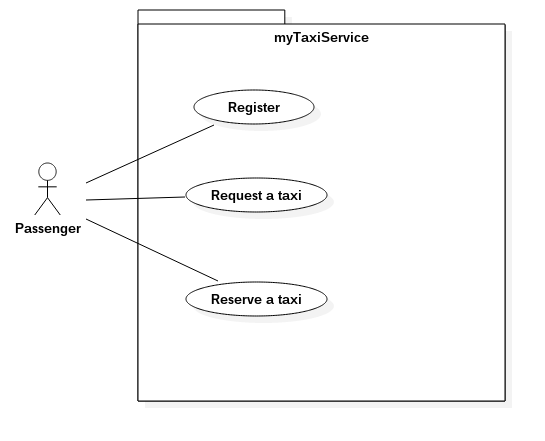
\includegraphics[scale=0.5]{Images/uc_highLevel_passenger}
\end{figure}
\subsection{Functions for Taxi Drivers}
A Taxi Driver can:
\begin{itemize}
\item Start his working activity by putting himself as available
\item Accept an incoming request from a Passenger, both immediate requests and reservations
\item Refuse an incoming request from a Passenger, both immediate requests and reservations
\item Finish his working activity by putting himself as not available
\end{itemize}
\begin{figure}[H]
\centering
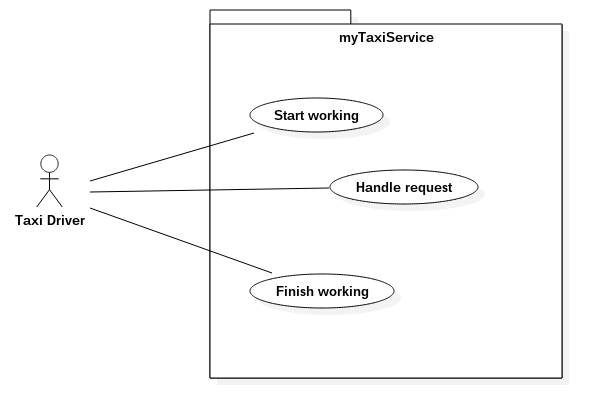
\includegraphics[scale=0.5]{Images/uc_highLevel_taxiDriver}
\end{figure}